\documentclass[a0,portrait]{a0poster}

\usepackage{multicol} % This is so we can have multiple columns of text side-by-side
\columnsep=100pt % This is the amount of white space between the columns in the poster
\columnseprule=3pt % This is the thickness of the black line between the columns in the poster

\usepackage[svgnames]{xcolor} % Specify colors by their 'svgnames', for a full list of all colors available see here: http://www.latextemplates.com/svgnames-colors

\usepackage{times} % Use the times font
%\usepackage{palatino} % Uncomment to use the Palatino font

\usepackage{graphicx} % Required for including images
\graphicspath{{figures/}} % Location of the graphics files
\usepackage{booktabs} % Top and bottom rules for table
\usepackage[font=small,labelfont=bf]{caption} % Required for specifying captions to tables and figures
\usepackage{amsfonts, amsmath, amsthm, amssymb} % For math fonts, symbols and environments
\usepackage{wrapfig} % Allows wrapping text around tables and figures

\usepackage{hyperref}
\hypersetup{
    colorlinks,
    linkcolor={red!50!black},
    citecolor={blue!50!black},
    urlcolor={blue!80!black}
}
\usepackage{cleveref}

\begin{document}

%----------------------------------------------------------------------------------------
%	POSTER HEADER 
%----------------------------------------------------------------------------------------

% The header is divided into two boxes:
% The first is 75% wide and houses the title, subtitle, names, university/organization and contact information
% The second is 25% wide and houses a logo for your university/organization or a photo of you
% The widths of these boxes can be easily edited to accommodate your content as you see fit

\begin{minipage}[b]{0.75\linewidth}
\veryHuge \color{NavyBlue} \textbf{Conflict Prediction with Spike and Slab prior} \color{Black}\\ % Title
\Huge\textit{}\\[2cm] % Subtitle
\huge \textbf{Anh Le}\\[0.5cm] % Author(s)
\huge Political Science Department\\[0.4cm] % University/organization
\Large \texttt{anh.le@duke.edu}\\
\end{minipage}
%
\begin{minipage}[b]{0.25\linewidth}

\includegraphics[width=20cm]{Duke-logo.jpg}\\
\end{minipage}

\vspace{1cm} % A bit of extra whitespace between the header and poster content

%----------------------------------------------------------------------------------------

\begin{multicols}{2} % This is how many columns your poster will be broken into, a portrait poster is generally split into 2 columns

%----------------------------------------------------------------------------------------
%	ABSTRACT
%----------------------------------------------------------------------------------------

\color{Navy} % Navy color for the abstract

%----------------------------------------------------------------------------------------
%	INTRODUCTION
%----------------------------------------------------------------------------------------

\color{SaddleBrown} % SaddleBrown color for the introduction

\section*{Introduction}

Being able to predict conflict is very useful for governments and international organizations to deploy their limited resources effectively. Therefore, this project will try to predict the (binary) presence of four events (i.e. insurgency, rebellion, dpc--domestic crisis, and erv--ethnic violence). I use monthly data of 167 countries from 2001 to present (dimension = $27,000 \times 550$). The feature variables include each country's politics, economic performance, financial status, and their 2-month lags.

The project will use logistic regression with spike-and-slab prior to choose a small subset of variables. This will isolate important predictive factors, facilitating model interpretation. Given high correlations between temporally lagged variables, sparse regression will also avoid over-fitting. I will compare the predictive accuracy of this model against others currently used in our lab.

\color{DarkSlateGray} % DarkSlateGray color for the rest of the content

%------------------------------------------------

\section*{Analysis}

I pre-process the data by removing extraneous variables (country names, time ID, etc.) and, for each country in the dataset, add a binary variable that indicates whether an observation belongs to a country. This allows the model to have different intercepts for each country, essentially adding country fixed effect.

I fit the logistic model with spike-and-slab prior using the package \verb|BoomSpikeSlab|. To simultaneously fit four models for my four response variables, I use packages \verb|doMC| and \verb|foreach|. 

The model is trained on March2001-June 2013 data and tested on July2013-Sept2014 data. The results below come from a MCMC chain with $\text{iterations}=1000$ and $\text{burn-in}=100$. Even though the MCMC chain is not that long, due to the size of the dataset the computational time is already over 1.5 hour. 


\section*{Results}

\subsection*{Predictive performance}
\begin{itemize}
\item \autoref{tab:in_sample_performance} and \autoref{tab:out_sample_performance} show in-sample and out-sample predictive performance. As expected, in-sample fit is better than out-sample fit across all four events of interest.

\item The model can predict \textit{Insurgency} is predicted very well, but performs poorly in predicting \textit{DPC (domestic crisis)}. This is reflected in the ROC-curve shown in \autoref{fig:roc_insurgency} and \autoref{fig:roc_dpc}.
\end{itemize}

\begin{center}
% latex table generated in R 3.1.2 by xtable 1.7-4 package
% Fri Dec  5 14:50:23 2014
\begin{tabular}{rrrrrr}
  \hline
 & insurgency & rebellion & dpc & erv & mp \\ 
  \hline
brier & 0.005 & 0.006 & 0.042 & 0.008 & 0.036 \\ 
  auc.C & 0.996 & 0.999 & 0.927 & 0.989 & 0.764 \\ 
  precision & 0.981 & 0.957 & 0.789 & 0.961 & 0.548 \\ 
  recall & 0.767 & 0.769 & 0.410 & 0.681 & 0.068 \\ 
   \hline
\end{tabular}

\captionof{table}{In sample performance}
\label{tab:in_sample_performance}
\end{center}
%

\begin{center}
% latex table generated in R 3.1.2 by xtable 1.7-4 package
% Mon Dec  1 05:33:13 2014
\begin{tabular}{rrrrr}
  \hline
 & insurgency & rebellion & dpc & erv \\ 
  \hline
brier & 0.009 & 0.019 & 0.088 & 0.034 \\ 
  auc.C & 0.997 & 0.903 & 0.860 & 0.977 \\ 
  precision & 0.976 & 0.906 & 0.642 & 0.905 \\ 
  recall & 0.946 & 0.784 & 0.460 & 0.480 \\ 
   \hline
\end{tabular}

\captionof{table}{Out sample performance}
\label{tab:out_sample_performance}
\end{center}

\subsection*{Compare with old models}

\autoref{tab:out_sample_old_ebma_performance} shows the model currently used in our lab. It is a ensemble model of multiple themes (politics, economics, infrastructure, etc.). My new model performs better than this ensemble model across the board.  
\begin{center}
\begin{tabular}{rrrrr}
  \hline
 & insurgency & rebellion & dpc & erv \\ 
  \hline
brier & 0.06 & 0.03 & 0.12 & 0.03 \\ 
  auc.C & 0.94 & 0.97 & 0.78 & 0.93 \\ 
   \hline
\end{tabular}
\captionof{table}{Out sample ebma (old) performance}
\label{tab:out_sample_old_ebma_performance}
\end{center}

\autoref{tab:out_sample_old_benchmark_performance} shows performance benchmark from other labs. Again, my new model performs better than this benchmark, with the exception of recall on \textit{erv (Ethnic Violence)}
\begin{center}
\begin{tabular}{rrrrr}
  \hline
 & insurgency & rebellion & dpc & erv \\ 
  \hline
precision & 0.88 & 0.84 & 0.65 & 0.98 \\ 
recall & 0.78 & 0.86 & 0.47 & 0.71 \\ 
   \hline
\end{tabular}
\captionof{table}{Out sample benchmark (old) performance}
\label{tab:out_sample_old_benchmark_performance}
\end{center}

\begin{center}
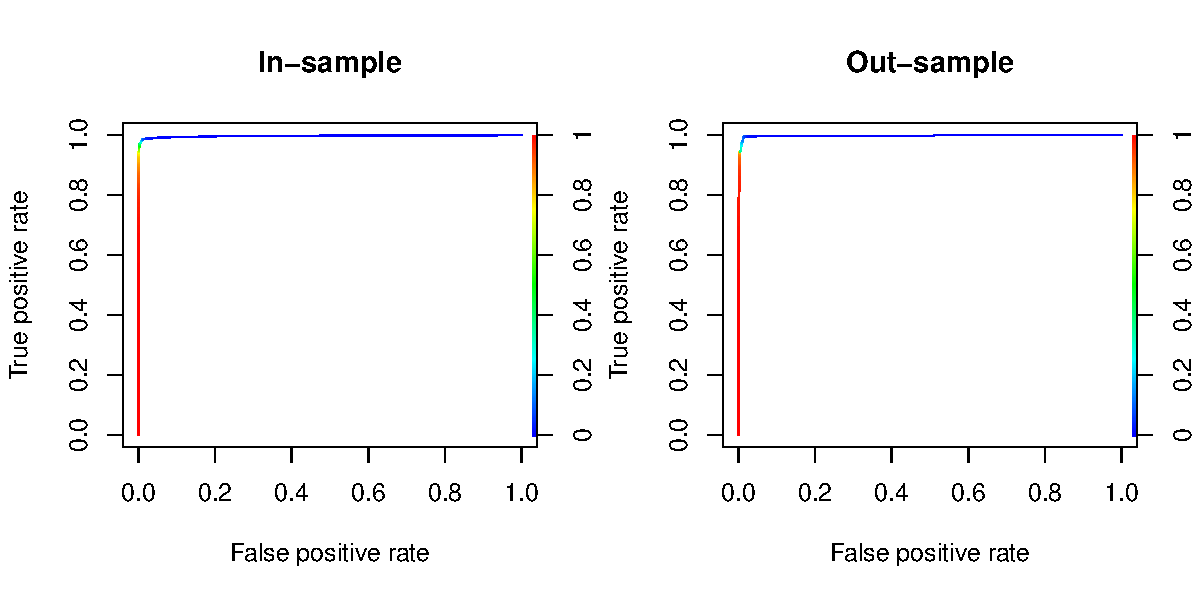
\includegraphics[width=0.5\textwidth]{roc_insurgency}
\captionof{figure}{ROC-curve of Insurgency}
\label{fig:roc_insurgency}
\end{center}

\begin{center}
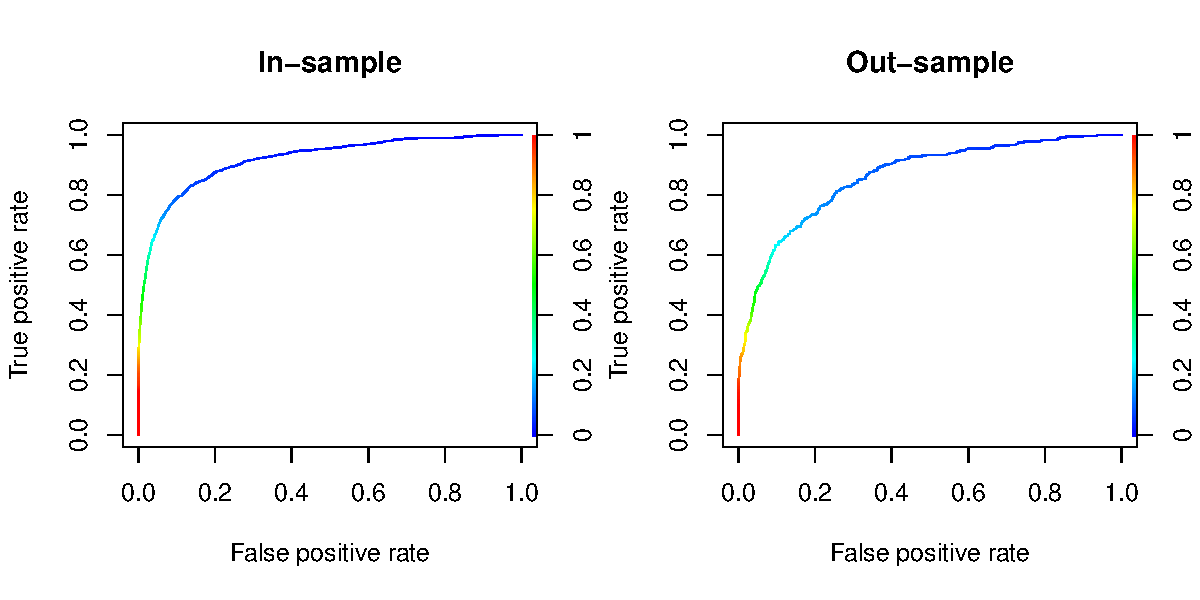
\includegraphics[width=0.5\textwidth]{roc_dpc}
\captionof{figure}{ROC-curve of DPC (Domestic Crisis)}
\label{fig:roc_dpc}
\end{center}

\subsection*{Variable selection}

\autoref{fig:variable_selection} shows the list of variables with positive inclusion probability. From 594 variables in the original dataset, there are only fewer than 40 variables left, achieving model sparsity.

However, we also recognize that most of the included variables are the binary country variable. This means that certain countries almost always (never) experience violence, crisis, etc. Therefore, it is a safe bet to predict that such countries will (not) have those events again.

Besides the country dummies, there are several factors crucial to predicting \textit{insurgency}:
\begin{itemize}
\item W.gower.events.rebellion.l1: Spatial-temporal 1 month lag of variable rebellion based on Gower distances (-)
\item AG.LND.TOTL.K2.l1: Land area (sq. km), lagged by 1 month (-)
\item State.Dept..l1: State Department Political Terror Scale, 1-month lag (+)
\item MS.MIL.TOTL.P1.l36: Total military expenditures in 2009 US dollars, lagged by 3 years (-)
\end{itemize}

\begin{center}
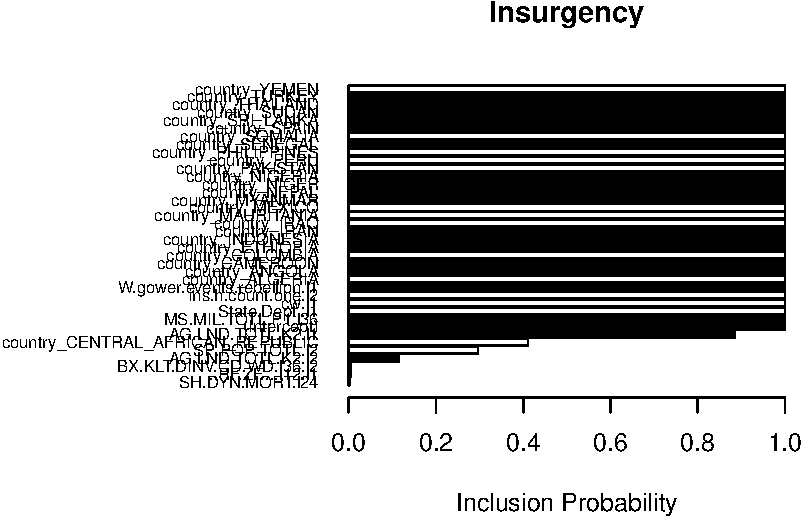
\includegraphics[width=0.5\textwidth]{variable_selection}
\captionof{figure}{Variables with Positive Inclusion Probability}
\label{fig:variable_selection}
\end{center}



%----------------------------------------------------------------------------------------
%	CONCLUSIONS
%----------------------------------------------------------------------------------------

\color{SaddleBrown} % SaddleBrown color for the conclusions to make them stand out

\section*{Conclusions}

\begin{itemize}
\item Logistic regression with spike-and-slab prior results in a sparse model with good performance. Even though the dataset has many lagged variables that are highly correlated, the spike-and-slab prior does a good job of selecting only one among them.
\item Most of the predictive performance comes from country fixed effects. This leads to better results than existing models, but does not give insights into which substantive factors leads to the events of interest. This probably means that the model won't be able to predict drastic change in a country.
\end{itemize}

\color{DarkSlateGray} % Set the color back to DarkSlateGray for the rest of the content

%----------------------------------------------------------------------------------------
%	FORTHCOMING RESEARCH
%----------------------------------------------------------------------------------------

\section*{Forthcoming Research}

\begin{itemize}
\item Model without country dummies
\item Focus on predicting moments of change
\end{itemize}

\end{multicols}
\end{document}